\section{Volba databázového systému}
\label{sec:implementation:db_choice}

Při návrhu bylo nutné zvolit konkrétní systém pro správu databáze. Nejprve bylo rozhodnuto o~typu databáze, a~poté byl vybrán konkrétní systém.

\subsection{Relační vs.\ dokumentová databáze}
\label{subsec:database:relational_vs_document}

Prvním rozhodnutím byl výběr mezi dokumentovou a~relační databází. Dokumentová databáze nabízí větší flexibilitu a~umožňuje ukládat celé \JSON odpovědi bez striktní struktury, avšak pro účely tohoto systému byla zvolena relační databáze.

Důvodem je analytická povaha dotazů a~potřeba agregovat data přes více entit. Relační databáze umožňuje efektivní spojování tabulek a~skupinové operace, které jsou v~nich dobře optimalizovány. Díky primárním a~cizím klíčům navíc zajišťuje integritu dat a~předem definovaná struktura zjednodušuje validaci a~konzistenci na straně aplikace.

\subsection{SQLite}
\label{subsec:implementation:db_choice:sqlite}

SQLite je odlehčený souborový databázový systém bez samostatného serverového procesu~\cite{sqlite_about}. Celá databáze je uložena v~jediném souboru a~databázový stroj je vložen přímo do aplikace jako knihovna. Tím odpadá nutnost instalace serveru, čímž se výrazně zjednodušuje lokální vývoj a~nasazení. SQLite je proto vhodné zejména pro prototypování, nízkou souběžnost nebo jako vestavěná databáze mobilních a~desktopových aplikací~\cite{sqlite_when_to_use}.

Nevýhodou je omezená podpora souběžných zápisů. Ve výchozím režimu (Rollback Journal) dochází při zápisu k~uzamčení celého souboru. Tento problém částečně řeší \WAL režim (\code{PRAGMA journal\_mode=WAL;})~\cite{sqlite_wal}, který umožňuje souběžné čtení za probíhajícího zápisu, avšak souběžné zápisy jsou stále serializovány. Nasazení ve vícekontejnerovém prostředí je kvůli sdílenému souboru problematické. Moderní cloudové platformy jako \devTool{Cloudflare D1}{https://developers.cloudflare.com/d1/} nebo \devTool{Turso}{https://turso.tech} tato omezení řeší, avšak SQLite má stále omezenější sadu analytických \SQL funkcí.

\subsection{PostgreSQL}
\label{subsec:implementation:db_choice:postgresql}

PostgreSQL je plnohodnotný serverový relační databázový systém~\cite{postgresql_about} fungující na architektuře klient-server. Umožňuje souběžný přístup více klientů, pokročilou správu transakcí a~efektivní využití systémových prostředků. Lokální nastavení vyžaduje spuštění serveru, které lze zjednodušit kontejnerizací. V~cloudu je PostgreSQL dostupný jako spravovaná služba u~všech hlavních poskytovatelů (Amazon RDS, Google Cloud SQL, Azure). Oproti vestavěným databázím zavádí architektura klient-server přídavnou síťovou latenci (\TCPIP), která je však při dávkovém zápisu zanedbatelná.

\subsection{Výsledné rozhodnutí}
\label{subsec:implementation:db_choice:decision}

Pro implementaci byl zvolen PostgreSQL. Rozhodujícím argumentem byla podpora analytického \SQL, zejména klauzule \code{DISTINCT ON}~\cite{postgresql_distinct_on}, kterou SQLite nenabízí a~která zjednodušuje dotazy typu point-in-time pro zjištění stavu každého \PR v~daném okamžiku. PostgreSQL dále poskytuje pokročilejší okenní funkce~\cite{postgresql_window_functions} pro výpočty nad časovými řadami a~propracovaný plánovač dotazů s~podporou různých typů indexů. Cloudové platformy moderního ekosystému SQLite tyto analytické konstrukty nativně nepodporují. Zatímco SQLite serializuje souběžné zápisy i~v~\WAL módu, PostgreSQL díky MVCC (multiversion concurrency control) a~zamykání na úrovni řádků zvládá zápisy lépe.

Pro lokální vývoj je server spouštěn přes kontejnerizaci, takže vývojář nemusí instalovat PostgreSQL přímo do systému a~vývojové prostředí zůstává shodné s~produkčním nasazením.

Srovnání obou systémů shrnuje \customref{Tabulka}{tab:implementation:db_choice:comparison}.

\begin{table}[htbp]
  \centering
  \caption{Srovnání vlastností SQLite a~PostgreSQL pro účely analytického nástroje}
  \label{tab:implementation:db_choice:comparison}
  \begin{tabularx}{\textwidth}{@{} l >{\raggedright\arraybackslash}X >{\raggedright\arraybackslash}X @{}}
    \toprule
    & \multicolumn{2}{c}{\textbf{Databázový systém}} \\
    \cmidrule(lr){2-3}
    \textbf{Kritérium} & \textbf{SQLite} & \textbf{PostgreSQL} \\
    \midrule
    Architektura & Vestavěná knihovna. & Klient-server architektura. \\
    \addlinespace
    Lokální nasazení & Zcela bezúdržbové, stačí jeden soubor. & Vyžaduje instalaci serveru nebo spuštění přes kontejnerizaci. \\
    \addlinespace
    Cloudové nasazení & Tradiční kontejnerové nasazení problematické; moderní platformy (D1, Turso) řeší omezení, avšak s~omezenější sadou analytických \SQL funkcí. & Nativní podpora, dostupné jako spravovaná služba. \\
    \addlinespace
    Souběžné zápisy & Ve výchozím režimu zamyká celý soubor; \WAL mód serializuje souběžné zápisy. & Plná podpora souběžnosti a~nezávislých transakcí. \\
    \addlinespace
    Analytické dotazy & Chybí \code{DISTINCT ON} a~pokročilé okenní funkce. Vhodné pro jednodušší dotazy. & Pokročilý optimalizátor, \code{DISTINCT ON}, okenní funkce a~bohatá podpora datových typů. \\
    \bottomrule
  \end{tabularx}
\end{table}

\section{Struktura databáze}
\label{sec:database}

Při návrhu struktury databáze bylo klíčové zajistit, aby schéma efektivně pojmulo velké množství dat a~zároveň umožňovalo rychlé provádění analytických dotazů.

\subsection{Rozdělení štítků a~událostí}
\label{subsec:database:labels_and_events}

Každý \PR a~issue má dvě kategorie historických změn. První kategorií jsou \emph{události} -- akce jako sloučení, uzavření, znovuotevření, přidání komentáře a~podobně, které jsou reprezentovány typem události a~časovým razítkem. Druhou kategorií jsou \emph{štítky} -- metadata přiřazovaná k~\PR nebo issue (například \code{S-waiting-on-review}), u~nichž je nutné sledovat štítek, časové razítko a~zda byl štítek přidán nebo odebrán. Tyto štítky se sledují především kvůli sledování stavů \sectionref{sec:rust_labels}.

Ukládání kompletní historie událostí a~štítků je nezbytné pro správné fungování dotazů Q1, Q2 a~Q4 \subsectionref{subsec:requirements:queries}, které rekonstruují historický stav~\PR a~issues k~zadanému datu. Bez těchto dat nelze přesně zpětně určit, v~jakém stavu se daný~\PR nacházel v~konkrétním okamžiku.

Protože události a~štítky mají odlišné atributy a~slouží jiným analytickým účelům, jsou uloženy ve dvou samostatných tabulkách: \code{issue\_event\_history} a~\code{issue\_labels\_history}. Jejich sloučení do jedné tabulky by vyžadovalo volitelné sloupce pro atributy druhého typu, nebo by vedlo k~redundanci dat.

\subsection{Diagram databáze}
\label{subsec:database:database_diagram}

Celková struktura databáze je znázorněna na \customref{Obrázku}{fig:database:overall_database}. Schéma má tři hlavní logické části: strukturu přispěvatelů a~přiřazení do týmů, aktuální stav \PR a~issues a~historii změn issues zahrnující zaznamenané události, změny štítků a~soubory upravené v~rámci sloučených nebo uzavřených \PR.

\begin{figure}[H]
  \centering
  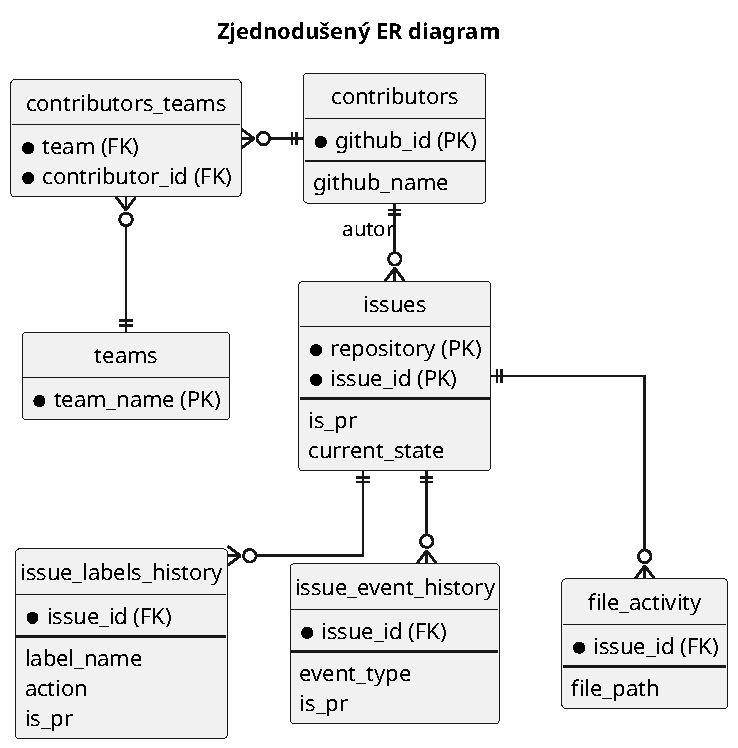
\includegraphics[width=0.7\textwidth]{figures/architecture/overall_database.pdf}
  \caption{Celkový přehled databázového schématu}
  \label{fig:database:overall_database}
\end{figure}

Podrobnější ER diagram databáze je uveden v~příloze \imageref{fig:appendix:database}. Centrem schématu je tabulka issues, která obsahuje aktuální stav issue i~\PR. Tato tabulka je společná pro oba typy záznamů, protože i~na straně GitHubu je každý \PR zároveň issue a~rozlišení probíhá pouze pomocí příznaku. Například u~endpointu pro získání issues se rozdíl mezi \PR a~issue pozná primárně pomocí přítomnosti pole \code{pull\_request} v~objektu entity v~odpovědi. Kvůli tomuto jedinému rozdílu je na tabulce implementován podmíněný index, konkrétně dva: jeden pro záznamy, kde \code{is\_pr = true}, a~druhý, kde \code{is\_pr = false}. Tento index efektivně rozděluje prohledávání tabulky na dvě části, čímž zmenšuje jeho velikost a~urychluje vyhledávání.

Do historických entit jsou pouze přidávány nové události a~záznamy jsou neměnné. Ostatní záznamy v~tabulkách jsou aktualizovány podle posledního známého stavu.

Data o~týmech jsou sice dostupná přes Team \API \sectionref{sec:rust_team_api} jako jednorázová \JSON odpověď, avšak pro analytické dotazy Q6 a~Q7 \subsectionref{subsec:requirements:queries} je nutné je mít v~databázi. Tyto dotazy vyžadují \SQL \code{JOIN} tabulky \code{file\_activity} s~přiřazením přispěvatelů do týmů. Bez lokálních dat by bylo nutné při každém dotazu volat Team \API a~filtrovat výsledky v~aplikační vrstvě. Data jsou proto uložena do tabulek \code{teams} a~\code{contributors\_teams} a~obnovována při každé synchronizaci, aby odrážela aktuální složení týmů.

Vztah mezi týmem a~přispěvatelem je realizován jako vazba m:n přes spojovací tabulku \\ \code{contributors\_teams}, protože každý člen může být ve více týmech a~každý tým má více členů.

Ohledně souborů je zaznamenáváno pouze to, kdo daný soubor upravil, konkrétní provedené změny se neukládají. Tabulka \code{file\_activity} slouží jako základ pro dotazy Q5, Q6 a~Q7 \subsectionref{subsec:requirements:queries}. Cílem těchto dotazů je zjistit, na jakých částech projektu se daný přispěvatel nebo tým podílel, nikoli sledovat konkrétní upravené funkcionality.
